% -*-latex-*-
% Document name: display.tex
% Creator: Rob MacLeod [macleod@vissgi.cvrti.utah.edu]
% Last update: September 2, 2000 by Rob MacLeod
%    - created
% Last update: Sun Sep 24 22:24:02 2000 by Rob MacLeod
%    -  Version 5.0Beta release edition
% Last update: Mon Jul 23 13:28:30 2001 by Rob MacLeod
%    - release 5.2
% Last update: Fri Jun 21 13:35:32 2002 by robmacleod
%    - late update for release 5.3
% Last update: Wed Mar 31 13:35:32 2004 by Bryan Worthen
%    - late update for release 6.0
% Last update: Wed Jun 30 13:28:30 2004 by Bryan Worthen
%    - release 6.1
% Last update: Wed May 11 13:28:30 2005 by Bryan Worthen
%    - release 6.3
%%%%%%%%%%%%%%%%%%%%%%%%%%%%%%%%%%%%%%%%%%%%%%%%%%%%%%%%%%%%%%%%%%%%%%
%%%%%%%%%%  Figures used in this file %%%%%%%%%%%%%%%%%%%%%%%%%%%%%%%%
%begin{latexonly}
  \newcommand{\timesignal}%
  {\centerline{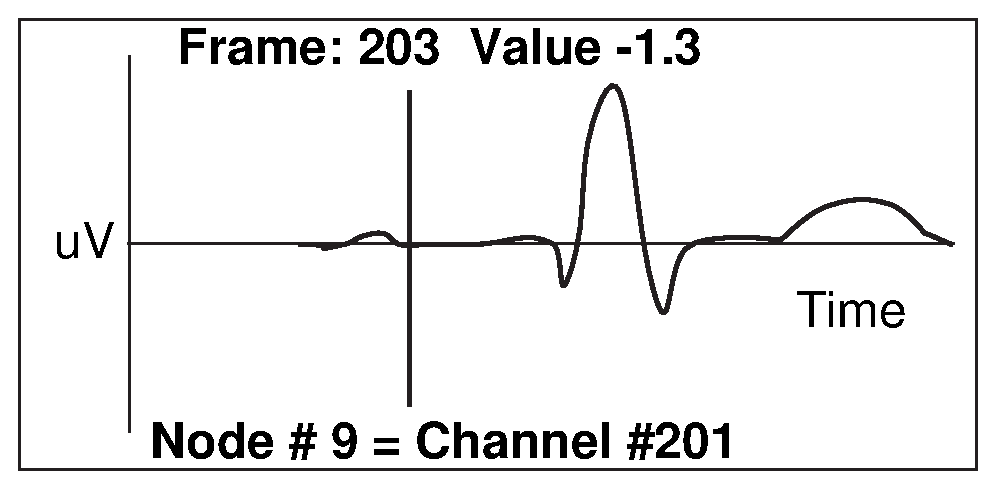
\includegraphics[height=2in,
  bbllx=165, bblly=197, bburx=627, bbury=415]{figures/timesignal.eps}}}
%end{latexonly}
\begin{htmlonly}
  \newcommand{\timesignal}{%
  \htmladdimg[align=top,width=714,alt="time signal"]
  {../figures/timesignal.gif}}
\end{htmlonly}
%%%%%%%%%%%%%%%%%%%%%%%%%%%%%%%%%%%%%%%%%%%%%%%%%%%%%%%%%%%%%%%%%%%%%%

\section{Display features}
\label{sec:display} 

This section describes the displays that \map{} generates and what they
mean; for specific information on how to control \map{} and the displays,
see Section~\ref{sec:control}.

\subsection{Multiple surfaces}
\label{sec:displaysurfaces} 

The idea of \map{} has always been to display multiple sets of data on
multiple surfaces; the limitation has been how much flexibility to include
in a single invocation of the program.  This version of \map{}, as opposed
to previous versions, can now handle multiple windows each with multiple
surfaces.  Surfaces can be moved between windows (see
Section~\ref{sec:fileswindow}) When \map{} displays multiple surfaces, each
can exist in its own full window with its own border and window title bar,
or, \map{} can build a single main window with multiple sub-windows inside
the main window.  The user can reposition and resize each of these
sub-windows using the Alt(Meta) key and the left and middle mouse buttons
respectively.  To create this layout of main window and frameless
sub-windows, use the \texttt{-b} (borderless windows) option when launching
\map{} as described in Section~\ref{sec:usage-geometry}.


\subsection{Surface display }

The basic forms of display of the surfaces are
%
\begin{itemize}
  \item nodes or points from each surface
  \item connectivity mesh
  \item shaded surfaces based on either the geometry or the associated
        scalar values, with a number of different rendering options.
  \item landmarks superimposed on the surface display
\end{itemize}

%%%%%%%%%%%%%%%%%%%%%%%%%%%%%%%%%%%%%%%%%%%%%%%%%%%%%%%%%%%%%%%%%%%%%%

\subsection{Mesh Rendering}
\label{sec:display-mesh} 

Often the purpose of \map{} is to render a geometry consisting of nodes and
connectivities and there are several basic modes of rendering this
information. 

\begin{description}
  \item [Points: ] display just the nodes of the geometry as dots or marked
        with spheres.
  \item [Connectivities: ] display the connectivity information for the
        mesh as lines joining the nodes.
  \item [Elements: ] treat each polygon in the mesh as an element and
        render it in a way that shows its surface; for triangles, simple
        render each triangle surface; for tetrahedra there is no specific
        rendering in this version of \map{}.
  \item [Elements and connectivities: ] \map{} also supports a hybrid mode
        of rendering that shows outward facing triangles (using the
        convention of counterclockwise ordering) as elements but backwards
        facing triangles as connectivities.
\end{description}

\map{} also has the ability to render
all elements with a lighting model.  This is especially useful for
displaying the elements of the mesh.  Additional controls to note are depth
cueing, which can reveal the depth relationships between elements of the
mesh. 

%%%%%%%%%%%%%%%%%%%%%%%%%%%%%%%%%%%%%%%%%%%%%%%%%%%%%%%%%%%%%%%%%%%%%%

\subsection{Surface Data Display} 
\label{sec:display-data} 

The main use of \map{} is to display scalar data associated with geometry
and there are numerous options and controls to facilitate this.  The two
basic ways of conveying scalar value information are as shaded surfaces
and contour lines and \map{} supports each separately, as well as in
combination.  For surface shading, there are several basic rendering modes:

\begin{description}
  \item [Flat: ] each triangle received a single color that depends on the
        mean value of the scalar value over that triangle.
  \item [Gouraud: ] the colour of each triangle values linearly with the
        value at each of the vertices.  The current version uses texture
        mapping to achieve more desirable results, but if your hardware
        does not support texture mapping, you can toggle it with the g-key.
  \item [Banded: ] the regions between contour lines have a constant color,
        even if the contour lines are not visible.
  \item [Contours: ] this can be a separate rendering mode, or combined
        with any of the three modes above.  Contours are lines that trace
        iso-values over the surface of the geometry.
\end{description}


\subsubsection{Data scaling}
\label{sec:scaling} 

There is a wide variety of options available for mapping scalar values to
colour and contour levels.  One can picture the process as based on four
facets: 

\begin{description}
  \item [Extrema: ] the extrema of the data and the selected colour maps
        determine the basic parameters of how value maps to color.  \map{}
        maintains a detailed list of data extrema organized both by time
        signal, time instant and by surface.  Thus it is possible to determine
        extrema based on just the most local of conditions---a particular
        frame and surface---or by more global conditions---the full range
        of frames or the full set of surfaces.
  \item [Scaling function: ] the mapping between value and color occurs
        according to some mathematical function, the simplest of which
        is linear.   The scaling function uses the selected extrema and
        describes a complete mapping between value and color.
  \item [Mapping: ] by scale mapping, we mean how the translation from
        value to color treats positive and negative values.  We may choose
        to map uniformly between the extrema or to apply different
        extrema or functions to the positive and negative values.
  \item [Color maps: ] the color displayed for a particular scalar value
        depends on the actual range of colors and their order in the color
        map.
\end{description}

\map{} can adjust all four facets of the scaling to create a wide range of
displays.  Note that all surfaces conform to the first three scaling
options (there is only one scaling range, function, and mapping that
corresponds to all surfaces).  We also chose to limit some of these 
options, however, in an effort
to create reproducible displays that reflect standard within the field.  Of
course, we chose our field, electrocardiography, as the basis, a fact for
which we make no apologies and simply encourage others to make similar
choices for their own field and implement \map{} accordingly.  Subsequent
versions of \map{} will support this flexibility.

Below are the specific choices that \map{} offers to control data scaling
and display
\begin{description}
  
  \item[Scale range] \map{} supports several selections of range over which
    to look for extrema.  In {\em local\/} range, only the data presently
    visible are scanned for extrema---this is the default.  In the full
    {\em global\/} range, all the data in the entire dataset are used, even
    those not presently visible on the display.  In between these cases,
    one can have global in time and local in space, \ie{} we scale each
    surface separately but use all time values for that surface.  Or one
    can select local in time and global in space, in which \map{} scans all
    surfaces for the data extrema, but for each time instant separately.  

    The user can also select group
    scaling, where he assigns surfaces to groups and the range is based on
    the group min/max (either local in time or global).  Groups are
    assigned by the menu.  The user can also do slave scaling, where he
    assigns one surface (slave) to another's (master) range.  The slave
    surfaces are currently only set through the command line, by placing a
    -sl num (where num is the surface number of the master) after declaring
    the slave surface.  See Section~\ref{sec:control-menus} and
    Section~'ref{sec:scalarparams} for details.

    If these options are not suitable, the user can select his own scaling 
    scope for
    maximum and minimum values. This can be set via the command line 
    (see {\tt -pl} and {\tt -ph} input parameters in Section~\ref{sec:usage}).
    or in the Contour Spacing dialog (see Section~\ref{sec:contourwindow}).
    While the rest of the scaling range options are set once for all 
    surfaces, whether or not an individual surface corresponds to the
    default range can be selected through the Contour Spacing dialog as well.

        
  \item[Scale function] The scale model describes the way in which scalar
    data are mapped to colours (or contours).  The present choice is
    linear, but the next version of \map{} will include: \textbf{linear}
    model, which simply maps the data to a range of colours in a completely
    linear fashion, \ie{} \mbox{$colour = K \phi$}; the
    \textbf{logarithmic} model, which highlights the lower level data
    values at the cost of poorer resolution at the higher levels \ie{}
    \mbox{$colour = A\log(\phi) + B$}; and the \textbf{exponential} model,
    which does the opposite, compressing the smaller levels and expanding
    the higher ones to span a wider colour range, \ie{} \mbox{$colour = A
      e^{B\phi}$}.
    
    The two schemes with fixed numbers of contours, {\em log/7-levels\/}
    and {\em log/13-levels\/} both map the upper decade ($\phi_{max}$ to
    $\phi_{max}/10.$) of the potential data range into a fixed set of
    logarithmically spaced values.  These values are composed of a mantissa
    from the standard E6 (1.0, 1.5, 2.2, 3.3, 4.7, 6.8, and 10.) and E12
    (1.0, 1.2, 1.5, 1.8, 2.2, 2.7, 3.3, 3.9, 4.7, 5.6, 6.8, 8.2, and 10.)
    number series, and an exponent such that the largest mantissa falls
    into the range 1.0 to 10. Hence as long as the extrema is known, it is
    possible to read absolute values from the individual contour lines.
    
  \item[Scale Mapping] There are several different ways to manage the way
    positive and negative data are treated in the scaling transformations
    in \map{}.  The current version supports the simplest, or {\em true\/}
    mapping, in which the data are used as they are with no consideration
    of positive or negative values---the color map spreads evenly across
    the range of the extrema.  Subsequent versions will support the {\em
      symmetric\/} scale mapping, which sets the positive and negative
    extrema symmetrically---the larger (in the absolute value sense)
    determines both maximum and minimum data values.  Also to appear in the
    net version is the {\em separate\/} scale mapping, in which the
    positive and negative extrema are treated completely
    separately---`half' the colours (and contours) are used for the
    positive values, half for the negative values.  This is equivalent to
    producing maps with the same number of contours for both positive and
    negative values, even when the positive data have a different absolute
    maximum value than the negative data.
    
  \item[Colour Map] There are four different colour maps presently
    implemented with every chance of more to come. The user can select
    which colour map to use. The choices currently implemented are:
        %
    \begin{description}
        
      \item [Jet map] (default) The Jet map is the same as the one 
        used in Matlab. Colours range from dark
        blue (for negative extrema) through greens (near zero)
        to dark red (positive extrema).  Jet utilizes a minimal set of similar
        color, particularly of greens and yellows, a complaint of the 
        Rainbow map.

      \item [Rainbow map] Colours range in rainbow fashion from
        blue (for negative extrema) through greens (near zero)
        to red (positive extrema).
        
      \item [Red (+) to Green (-)] Largest negative value is coloured
        bright green, dark grays are for the region near zero, and
        positive values appear red. 
        
      \item [Black (+) to White(-)] Grey shades from black for small
        values to white for large ones.
        
    \end{description}
      Note that for each color map, the direction of the mapping to value
      can be inverted, \eg{} in the default directions, blue indicates
      small or negative values and red indicates large or positive values.
      Inverted, this map uses red for small values and blue for large
      values.
      
  \item[Contours] 
    Contours will be spaced according to the scaling parameters mentioned
    above.  The number of contours or contour spacing can be changed in the
    Contour Dialog (See Section~\ref{sec:contourwindow}).  If 'contour 
    spacing' is selected, the spacing will determine the number of contours
    based on the range.  If the function is linear and the mapping is true,
    the gap between contours will be the number specified in the dialog.
    
    
\end{description}

\subsubsection{Scalar data reference}
\label{sec:reference} 

Related to scaling is the reference channel used for the displayed scalar
data.  By default, we assume that scalar values already have the right
reference and we do nothing to change that.  The user can, however, select
a new reference and then subtract that reference from all signals in the
surface.  This is done by selecting the ``Reference lead - single value''
or ``Reference lead - mean value'' from the Picking menu (See
Section~\ref{sec:control-picking}).  There are at present two types of
references that \map{} supports:
\begin{description}
  \item[Mean as reference: ] Selecting the mean as reference causes \map{}
    to subtract the average value over each surface for each instant in
    time from the scalar data on that surface.  Selecting the ``Reference
    lead - mean value'' from the Picking menu automatically does this, and
    can be undone by selecting ``Reset Reference'' from the same menu.
    
  \item[Selected lead as reference: ] It is also possible to select a
    single channel of data and use that as the reference signal.  This is
    done by first entering the the pick mode called ``Reference lead -
    single value'', and then selecting the reference node (See
    Section~\ref{sec:control-mouse}) performs this operation.  The rest of
    the nodes then use that node as a reference value.  Selecting a new
    reference lead works properly, \ie{} the effect is not cumulative but
    first restores the data to the original state, than applies the new
    reference, and this can all be undone by selecting ``Reset Reference''
    from the same menu.
\end{description}


%%%%%%%%%%%%%%%%%%%%%%%%%%%%%%%%%%%%%%%%%%%%%%%%%%%%%%%%%%%%%%%%%%%%%%

\subsection{Landmarks}
\label{sec:landmarks}

Landmarks provide a means to include visual icons and markers in the
surface display in \map{}.  They are not meant to render realistically but
simply to be cues to assist the user in identifying perspective or features
of the surfaces.  The list of support landmarks reflects our current usage
for bioelectric field data from the heart but many of the landmark types
are general purpose and hence useful in other contexts.  

Section~\ref{sec:lmfile} describes the currently support landmark types
and the files that contain them.  Display of each landmark type depends on
the type and user controlled options (see Section~\ref{sec:control} for
details on controlling the display).

%%%%%%%%%%%%%%%%%%%%%%%%%%%%%%%%%%%%%%%%%%%%%%%%%%%%%%%%%%%%%%%%%%%%%%

\subsection{Clipping Planes}
\label{sec:clipping} 

Clipping planes allow you to remove from view certain parts of the display
so that you can better see what is left.  So everything on one side of the
clipping plane is visible and everything on the other is not.  

We have two clipping planes in \map{} and their position and alignments are
adjustable as well as their relation to each other---we can lock the
clipping planes together so they work like a data slicer, always showing a
slice of constant thickness.

The controls for clipping planes are adjustable from the menus (see
Section~\ref{sec:control-menus}) and also via keyboard controls (see
Section~\ref{sec:control-keys}.   The basic controls turn the two clipping
planes on and off, lock them together, and lock their position relative to
the objects in the surface display.  By unlocking the last control, you can
select that part of the display you want to clip; the default clipping
planes are along the z-axis of the object (up and down).  To control
position of the planes along their normal direction, just keep hitting the
bracket keys ([] and \{\}).

%%%%%%%%%%%%%%%%%%%%%%%%%%%%%%%%%%%%%%%%%%%%%%%%%%%%%%%%%%%%%%%%%%%%
%%%%%%%%%%%%%%%%%%%%%%%%%%%%%%%%%%%%%%%%%%%%%%%%%%%%%%%%%%%%%%%%%%%%%%

%  \subsection{Perspective view and depth cueing}
%  \label{sec:perspective} 

%  In \map{} the default view mode is orthogonal and there is no depth
%  cueing.  Both can, however, be switched on at the user's request. To toggle
%  between orthogonal and perspective views, use the o-key.  Currently, the
%  modeling transformations (rotation, translation, scaling) are all reset
%  when you switch modes, but this will hopefully be handled better in the
%  future. Note that in perspective mode, scaling and translation can be used
%  to change the degree of perspective in the display. By moving the object
%  further away (with the translate dial) and then increasing the scaling, the
%  degree of perspective is reduced, while by pulling the object closer and
%  reducing the scaling, the opposite occurs. The use of the bounding cube
%  (see next section) can serve as additional visual feedback on the spatial
%  definition of the object in the display.

%  Depth cueing works by reducing the intensity of lines and points in the
%  display as a function of the distance from the viewer (eye location). The
%  distance from objects in the display to the viewer is stored in a separate
%  ``z-buffer'', which has a value for each pixel in the screen. Depth cueing
%  is useful when viewing geometries or objects which would otherwise
%  be drawn with constant colour, but is misleading and invalid when the
%  colour is already being used to convey other information ({\em e.g.,}
%  colour-coded contour lines). Hence, use depth-cueing at your own
%  discretion. At the moment (\today), depth cueing is only supported for
%  drawing points and lines in \map{}. It can be combined with perspective
%  view to get fairly realistic images of three-dimensional objects which are
%  drawn as a wire mesh or as points.

%  To control depth cueing, use the d-key to toggle, and two menu items in the
%  ``Set Clipping Plane'' menu to tune. The menu items ``Z-buffer near'' and
%  ``Z-buffer far'' allow the lower right (clipping plane) dial to be used to
%  move the front and back (near and far) z-buffer planes either closer to
%  (counterclockwise dial rotation) or farther from (clockwise rotation) the
%  viewer.  The trick to using this feature effectively is to note that when
%  the {\bf near} z-buffer plane moves through an object, ever pixel that is
%  in {\bf front} of it is drawn at full intensity (no depth cueing).  The
%  {\bf far} z-buffer plane has the opposite effect in that as it moves
%  forward through an object, pixels located {\bf behind} it are drawn at
%  minimal (often black or background) intensity.  The region between the two
%  z-buffer planes is spanned by the range of colour intensities which are set
%  in the program (currently 20 linear steps span the full range of each
%  colour).  Note that this is not the same effect as moving the clipping
%  planes around since the change in intensity is gradual, and the result
%  depends on which z-buffer plane is used. If the two z-buffer planes meet,
%  the object becomes invisible (for obvious reasons), a situation which
%  \map{} permits, but hardly encourages.

\subsection{Node marking}
\label{sec:displayleads} 

Node markings are just additional information added to the display of the
nodes.  This may be as simple as drawing spheres at the nodes to make them
more visible, or as elaborate as marking each node with its associated
scalar data value.  Section~\ref{sec:control-menus} describes these options
in detail.

%  There are many options for defining and marking a node in the geometry
%  display (and the lead or data channel associated with it).  This can lead
%  to ambiguity in the node labels and markings that appear in a display.  The
%  conventions used in \map{} are shown in the following table:
%  %
%  \begin{center}
%  \begin{tabular}{|l|p{1.3in}|p{1.3in}|p{1.3in}|} \hline
%  \multicolumn{4}{|c|}{Node number display conventions}\\ \hline
%  \multicolumn{1}{|c|}{\bf Node Marking} & 
%  \multicolumn{3}{|c|}{\bf Lead/channels file present}\\ \hline
%  & \multicolumn{1}{|c|}{None} &
%  \multicolumn{1}{|c|}{Channels} &
%  \multicolumn{1}{|c|}{Leadlinks} \\ \hline
%  Node numbers & same as in geometry files, starting at one for each surface
%  & unaffected  & unaffected \\ \hline
%  Lead numbers\footnotemark & same as in geometry files, consecutive over
%  all surfaces & channel numbers  & leadnumber from leadlinks info \\ \hline
%  Data values & potential value & potential value & potential value \\ \hline
%  \end{tabular}
%  \end{center}

%  \footnotetext{If both leadlink and channels information is present,
%  then leadlink has priority}

\subsection{Time signal display}
\label{sec:displayscalar}

Display option for the time signal are very modest in this version of
\map{}.  This will change\ldots{}

%  When the {\tt -t trace-lead-num} option is used, \map{} collects the data
%  from the incoming frames of map data and plots it as a time signal of the
%  data channel selected by the value of {\tt trace-lead-num}.  The value of
%  {\tt trace-lead-num} is interpreted in different ways depending on whether
%  {\em leadlinks\/} information (see Section~\ref{sec:leadfiles}) is present:
%  %
%  \begin{center}
%    \begin{tabular}{lll} \hline
%      \multicolumn{3}{c}{Selecting data channel for display} \\ \hline
%      \multicolumn{1}{l}{Leadlinks present} & 
%      \multicolumn{1}{l}{Channels present} & 
%      \multicolumn{1}{l}{Interpretation of trace-lead-num} \\ \hline
%      No & No & as node number \\ 
%      Yes & No & as a lead number \\
%      No & Yes & as a channel number \\
%      yes & Yes & as a channel number \\ \hline
%    \end{tabular}
%  \end{center}


Figure~\ref{fig:scalar} shows the layout and labeling of the scalar
window.  Font sizes adjust with the window size and the type of units may
be explicit if the time series data (\texttt{.tsdf}) files contain this
information. 

\begin{figure}[htb]
  \begin{makeimage}
  \end{makeimage}
  \timesignal
  \caption{\label{fig:scalar} Time signal window layout.  Vertical line
  indicates the frame currently displayed in the surface plot.   Text
  annotations can vary with the data content and mode settings.}
\end{figure}

For directions on how to control the time signal window, see
Section~\ref{sec:control-scalar}. 



%%% Local Variables: 
%%% mode: latex
%%% TeX-master: "manual"
%%% End: 
